\documentclass[10pt]{beamer}
\usepackage[utf8]{inputenc}
\usepackage{xeCJK}
\usepackage{graphicx}
\usepackage{mathtools}
\usepackage{utopia} %font utopia imported
\usepackage{geometry}
\usepackage{multimedia}
\usepackage{hyperref}
\usepackage{animate}
\usepackage{ragged2e}   %new code
\usepackage[spanish]{babel}
\usetheme{CambridgeUS}
\usecolortheme{dolphin}
\addtobeamertemplate{block begin}{}{\justifying}  %new code

% set colors
\definecolor{hkustyellow}{RGB}{167, 131, 55}
\definecolor{hkustblue}{RGB}{0, 56, 116}
\definecolor{hkustred}{RGB}{209, 51, 59}
\setbeamercolor*{palette primary}{bg=hkustblue, fg = white}
\setbeamercolor*{palette secondary}{bg=hkustred, fg = white}
\setbeamercolor*{palette tertiary}{bg=hkustyellow, fg = white}
\setbeamercolor*{titlelike}{fg=hkustblue}
\setbeamercolor*{title}{bg=hkustblue, fg = white}
\setbeamercolor*{item}{fg=hkustblue}
\setbeamercolor*{caption name}{fg=hkustblue}
\setbeamertemplate{caption}[numbered]
\usefonttheme{professionalfonts}
\usepackage{natbib}
\usepackage{hyperref}
%------------------------------------------------------------
\titlegraphic{
\includegraphics[height=2.5cm]{logoUA.png}}
% \usepackage{fontspec}
% \setmainfont{Times New Roman}


\setbeamerfont{title}{size=\large}
\setbeamerfont{subtitle}{size=\small}
\setbeamerfont{author}{size=\small}
\setbeamerfont{date}{size=\small}
\setbeamerfont{institute}{size=\small}
\setbeamertemplate{background}{%
    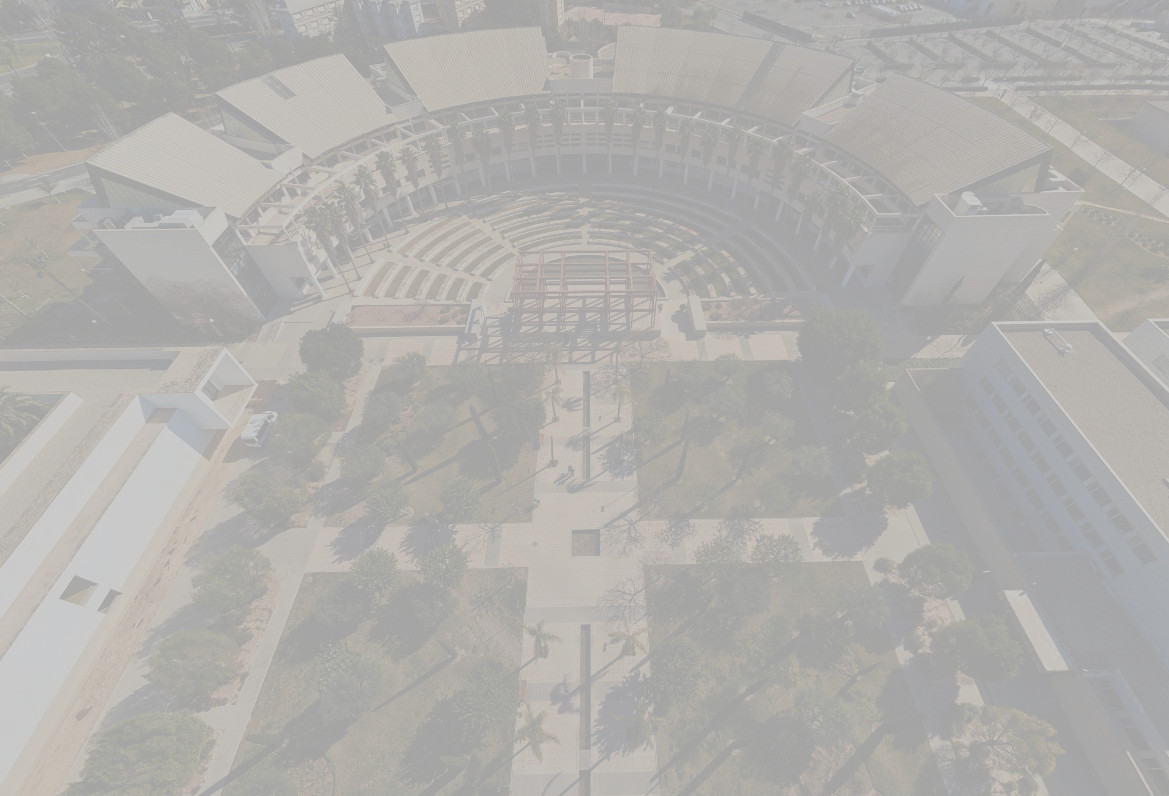
\includegraphics[width=\paperwidth,height=\paperheight]{aulario 2.jpg}
}

\title[Universidad de Alicante]{\textrm{\textbf{Práctica Demostrativa}}}
\subtitle{\textrm{Termomagnetismo}}
\author[vmr48@alu.ua.es y amhm10@alu.ua.es]{\textrm{Víctor Mira Ramírez y Ahlam Makboul Hilal}}

\institute[]{\textrm{Universidad de Alicante}}
\date[\today]{\textrm{\today}}

%------------------------------------------------------------
%This block of commands puts the table of contents at the 
%beginning of each section and highlights the current section:
%\AtBeginSection[]
%{
%  \begin{frame}
%    \frametitle{Contents}
%    \tableofcontents[currentsection]
%  \end{frame}
%}
\AtBeginSection[]{
  \begin{frame}
  \vfill
  \centering
  \begin{beamercolorbox}[sep=8pt,center,shadow=true,rounded=true]{title}
    \usebeamerfont{title}\insertsectionhead\par%
  \end{beamercolorbox}
  \vfill
  \end{frame}
}
%------------------------------------------------------------

\begin{document}

%The next statement creates the title page.
\frame{\titlepage}
\begin{frame}
\frametitle{\textrm{Índice}}
\tableofcontents
\end{frame}
%------------------------------------------------------------
\section{\textrm{Introducción}}
    \subsection{\textrm{Descripción del experimento}}
        \begin{frame}{\textrm{Descripción del experimento}}
            \begin{block}{Desarrollo experimental}
                El \href{https://youtu.be/rLcoyuIqBuM}{experimento} es simple: colocamos un clip cerca de un imán, atado a un alambre. Calentamos el clip con un soplete y observamos que el clip se despega del imán. Espontáneamente, al enfriarse, vuelve a sentirse atraido por el imán.
            \end{block}
            \begin{figure}
                \centering
                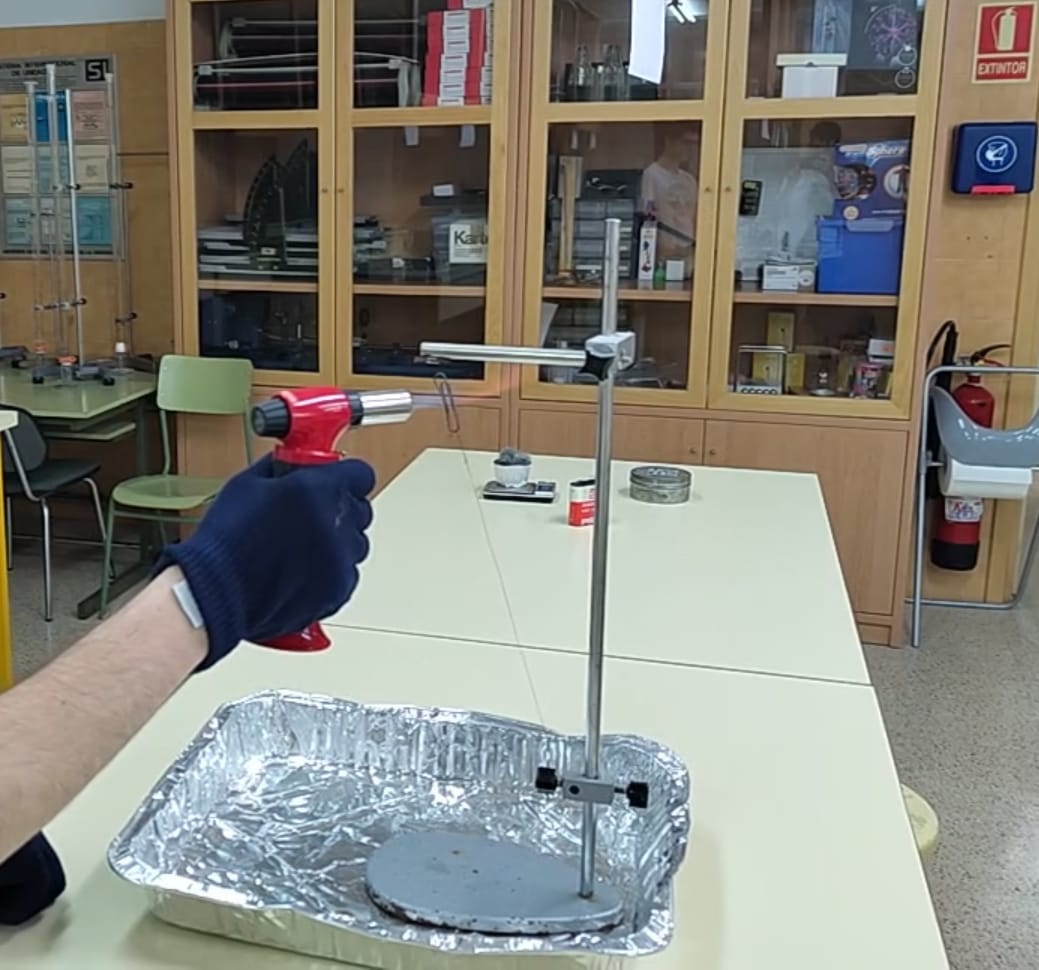
\includegraphics[scale=0.1]{experimento.jpeg}
                \caption{Aumento de la temperatura del clip bajo un campo magnético}
                \label{fig:experimento}
            \end{figure}
        \end{frame}
    \subsection{\textrm{Contexto histórico}}
    \begin{frame}{\textrm{Contexto histórico}}
        \begin{block}{Biografía}
            Pierre Curie (1859 - 1906) fue un físico francés, pionero en el estudio de la radiactividad, que fue galardonado con el Premio Nobel de Física en 1903 junto con Marie Curie y Antoine Henri Becquerel.
        \end{block}
        \begin{figure}
                \centering
                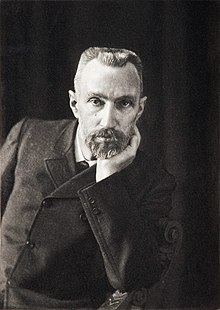
\includegraphics[scale=0.4]{pierre.jpg}
                \caption{Pierre Curie en 1906}
                \label{fig:dominio}
        \end{figure}        
    \end{frame}
    \begin{frame}
        \begin{block}{Descubrimientos}
            \vspace{0.4cm}
            \begin{itemize}
                \item \textbf{Principio universal de simetría (1894):}\\ Las simetrías presentes en las causas de un fenómeno físico también se encuentran en sus consecuencias. \vspace{0.4cm}
                \item \textbf{Piezoelectricidad (1908, junto a su hermano Jacques):}\\Fenómeno por el cual al comprimir un cristal de cuarzo se genera un potencial eléctrico y viceversa. \vspace{0.4cm}
                \item \textbf{Ley de Curie:}\\ Efecto de la temperatura sobre el paramagnetismo, conocido actualmente como la ley de Curie. \\También descubrió que las sustancias ferromagnéticas presentan una temperatura por encima de la cual pierden su carácter ferromagnético; esta temperatura se conoce como temperatura o punto de Curie.
            \end{itemize}             
        \end{block}
    \end{frame}

%------------------------------------------------------------
\section{\textrm{Hipótesis Inicial}}
    \begin{frame}{\textrm{Hipótesis Inicial}}
        \begin{block}{Hechos observables}
            \begin{itemize}
                \item El clip se calienta, y cae. 
                \item Relación calor/magnetismo. 
            \end{itemize}
        \end{block}
        \begin{block}{Hipótesis}
            Al calentar el clip, este pierde sus propiedades ferromagnéticas, y deja de ser atraído por el imán.
        \end{block}
    \end{frame}
%---------------------MARCO TEORICO-----------------------------
\section{\textrm{Marco Teórico}}
    \subsection{\textrm{Materiales Paramagnéticos y Ferromagnéticos}}
        \begin{frame}{\textrm{Materiales Paramagnéticos y Ferromagnéticos}}
            \begin{block}{Paramagnetismo}
                El paramagnetismo es el fenómeno que se da en el momento que las moléculas que se encuentran en una sustancia tiene un magnetismo estable.\vspace{0.3cm}\\ De la misma manera, aparece cuando los materiales se magnetizan cuando están en contacto con un campo magnético externo. \vspace{0.3cm}\\Este fenómeno aparece cuando algunos electrones no están emparejados.
            \end{block}
        \end{frame}
        \begin{frame}{\textrm{Materiales Paramagnéticos y Ferromagnéticos}}
            \begin{block}{Ferromagnetismo}
                El ferromagnetismo es una propiedad que poseen algunos materiales en los cuales los espines de los electrones que se conoce como dominio magnético se colocan paralelamente.\vspace{0.3cm}\\ En este caso la temperatura le afecta directamente ya que puede alterar el desorden si la temperatura se va incrementando, todos los materiales ferromagnéticos tienen una temperatura característica que se conoce como temperatura Curie $T_c$.
            \end{block}
            \begin{figure}
                \centering
                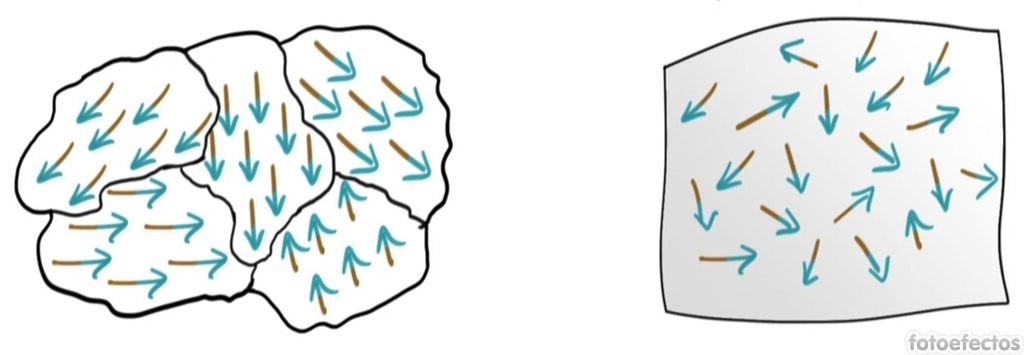
\includegraphics[scale=0.4]{fotoefectos.com_.jpg}
                \caption{Ferromagnetismo vs Paramagnetismo}
                \label{fig:dominio2}
            \end{figure}
        \end{frame}
        \begin{frame}{\textrm{Materiales Paramagnéticos y Ferromagnéticos}}
            \begin{block}{Dominio magnético}
            Los momentos magnéticos de todos los átomos de regiones casi macroscópicas se alinean formando micro imanes perfectos que se denominan dominios. Las orientaciones  de estas regiones son aleatorias y es por eso que generalmente aparecen desmagnetizados.
            \end{block}
            \begin{figure}
                \centering
                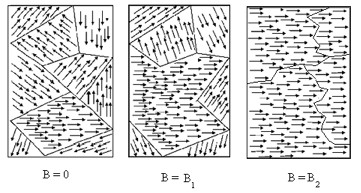
\includegraphics[scale=0.4]{dominio.jpg}
                \caption{Alineación de los dominios magnéticos}
                \label{fig:dominio1}
            \end{figure}
        \end{frame}





%---------------------TEMPERATURA DE CURIE-----------------------------

        
    \subsection{\textrm{Temperatura de Curie}}

    
    \begin{frame}{\textrm{Temperatura de Curie}} 
        \begin{block} {Temperatura de transición (Curie)}
            Ferromagnetismo  $\rightarrow$   Paramagnetismo
        \end{block}

        \vspace{1cm}
        \begin{block} {Ley de Curie}
            \begin{columns}
            \column{0.5\textwidth}
                \begin{equation*} 
                    \chi_m=\frac{C}{T}
                \end{equation*}
            \column{0.5\textwidth}
                Capacidad de un material paramagnético de magnetizarse
            \end{columns}       
        \end{block}
            
       
    \end{frame}
    
    \begin{frame}{\textrm{Temperatura de Curie}}
        \begin{block}{Ley de Curie-Weiss}
        \begin{columns}
            \column{0.5\textwidth}
             \begin{equation*}
                 \chi_m=\frac{C}{T-T_c}
             \end{equation*}
             \\
             \\
             \centering
                 (Aplicable a altas temperaturas)
            \column{0.5\textwidth}
                \begin{figure}
                    \centering
                    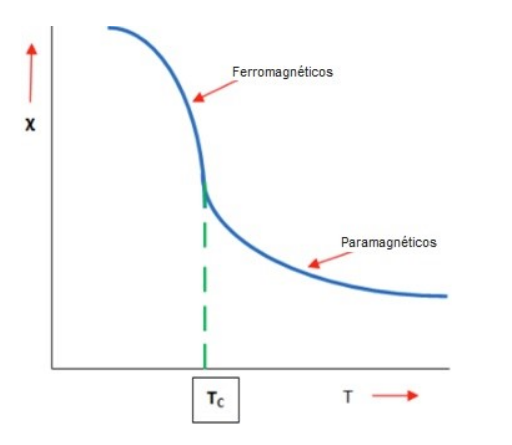
\includegraphics[scale=0.4]{Captura de pantalla (31).png}
                    \caption{Susceptibilidad/Temperatura}
                \end{figure}
     
        \end{columns}
            
        \end{block}
    \end{frame}

\begin{frame}{Cómo afecta la temperatura a nivel atómico}



\begin{block}{Desalineamiento de momentos magnéticos}
    
    $\uparrow$ T   $\rightarrow$     Agitación de los espines   $\rightarrow$     Desalineamiento de momentos

\end{block}

        \begin{figure}
            \centering
            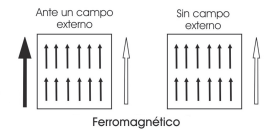
\includegraphics[scale=0.75]{ferro.png} 
            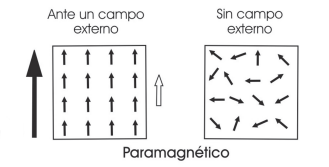
\includegraphics[scale=0.6]{para.png}
            \caption{Las flechas rellenas indican el campo aplicado y las vacías la magnetización del material bajo ausencia (der) o presencia (izq) de B según el tipo de material.}
            \label{fig:atom}
        \end{figure}

    \begin{center}
            \begin{block}{Acoplamiento de espines}
        $T < T_c$  $\rightarrow$   acoplados \\
        $T = T_c$  $\rightarrow$  $E_t=$ Energía acoplamiento\\
        $T > T_c$  $\rightarrow$   no acoplados 
            \end{block}

    \end{center}

    



    
\end{frame}
    
%---------------------------- APLICACION--------------------
\section{\textrm{Aplicación}}
       
    \subsection{\textrm{Funcionamiento del motor de Tesla}}
        \begin{frame}{Funcionamiento}
            \begin{block}{\href{https://youtu.be/mjI2AOjIJMs?t=88}{Ciclo del Motor de Tesla}}
                Objeto atraído por el imán.\\
                Se calienta hasta la Tª Curie\\
                Pierde sus propiedades ferromagnéticas.\\
                Se aleja del imán.\\
                Se enfría. \\
            \end{block}
            
            \begin{figure}
                \centering
                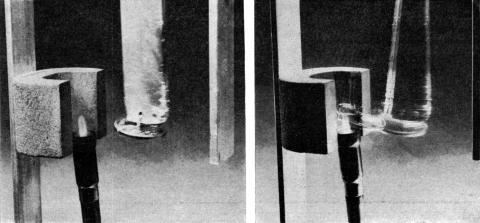
\includegraphics[scale=0.4]{image.png}
                \caption{Prototipo de Tesla}
                \label{fig:my_label}
            \end{figure}
        \end{frame}


            

%---------------------------- REFERENCIAS--------------------
\begin{frame}{Bibliografía y referencias}
    \begin{block}{Enlaces}
        \begin{itemize}
            \item \href{https://es.wikipedia.org/wiki/Ley_de_Curie}{Ley de Curie - Wikipedia}\\
            \item \href{https://es.wikipedia.org/wiki/Ley_de_Curie-Weiss}{Ley de Curie-Weiss - Wikipedia}\\
            \item \href{https://es.wikipedia.org/wiki/Pierre_Curie}{Pierre Curie - Wikipedia}
            \item \href{https://spiegato.com/es/que-es-la-temperatura-de-curie}{Temperatura de Curie - Spiegato}\\
            \item \href{https://teslauniverse.com/build/plans/teslas-thermomagnetic-motor}{Tesla's thermomagnetic motor - Arthur S. Cookfair}\\
            \item \href{https://edejesus.web.uah.es/resumenes/DECI/tema_4.pdf}{Magnetismo - UAH}
            \item \href{https://youtu.be/mjI2AOjIJMs}{Thermomagnetic Motor Based on The Curie Point - YouTube}\\
            \item \href{https://imamagnets.com/blog/diferencias-entre-materiales-ferromagneticos-paramagnetico-y-diamagneticos/}{Diferencias entre materiales ferromagnéticos, paramagnéticos y diamagnéticos}\\
            \item \href{https://es.wikipedia.org/wiki/Paramagnetismo}{Paramagnetismo - Wikipedia}\\
            \item \href{https://es.wikipedia.org/wiki/Ferromagnetismo}{Ferromagnetismo - Wikipedia}
            \item \href{https://app.ingemmet.gob.pe/biblioteca/pdf/LIB-230.pdf}{ASM - UNAM}
        \end{itemize}
    \end{block}
\end{frame}
    
%------------------------------------------------------------
\end{document}